\documentclass[conference]{IEEEtran}

% Language setting
% Replace `english' with e.g. `spanish' to change the document language
\usepackage[english]{babel}

% Useful packages
\usepackage{amsmath}
\usepackage{graphicx}
\usepackage{url}
\usepackage{float}

% Title and author info
\title{Analisis bibliografico - Reconocimiento facial}
\author{\IEEEauthorblockN{Sergio Peinado Cuevas - 506221009, Michael Esteban Castillo Lopez - 506221049}}

\begin{document}
\maketitle

\begin{abstract}
Resumen—In the contemporary era, Facial Expression Recognition (FER) plays a pivotal role in numerous fields due to its
vast application areas, such as e-learning, healthcare, marketing,
and psychology. FER involves analyzing facial features to identify
and verify individuals, making it a crucial area within artificial
intelligence (AI) and machine learning (ML). This technology has
applications ranging from security and surveillance to personalized services.
To explore this topic further, we conducted a comprehensive
and critical bibliographic analysis of various findings and projects
related to facial recognition. Our review included over 100
academic papers retrieved from Scopus. We identified common
themes, emerging trends, and advancements in FER. Additionally, we examined predominant methodological approaches,
including machine learning and deep learning techniques, face
detection, pre-processing, handcrafted feature extraction, and
emotion classifiers.
Challenges such as illumination, pose, and scale variation impact the accuracy of FER systems in controlled and spontaneous
facial expression datasets. Looking ahead, the development of
multimodal FER systems for real-time scenarios, considering
computational efficiency, remains an important avenue for enhancing system performance and reducing error rates.
\end{abstract}

\section{Introduction}

El reconocimiento facial, es una tecnologıa que ha ganado
una importancia significativa en las ultimas d ecadas, conso- 
lidandose como una de las areas mas innovadoras y desafian- 
tes dentro de la inteligencia artificial (IA) y el aprendizaje
automatico (ML). Esta tecnologıa permite la identificacion y 
verificacion de personas mediante el analisis de sus carac- 
terısticas faciales y tiene aplicaciones que abarcan desde la
seguridad y la vigilancia hasta la personalizacion de servicios. 
Por manejar temas tan utiles es que se decidio la eleccion de
este tema para la busqueda en la base de datos scopus, con la
finalidad de aprender mas sobre el tema y como esta busqueda
nos ayuda con estrategias e informacion para la realizacion de
nuestro proyecto de deteccion de fraude en examenes.
En este analisis bibliografico realizamos una revision
exhaustiva y crıtica de los diversos hallazgos y proyectos
sobre el reconocimiento facial. A traves de la recopilacion
y analisis de mas de 100 artıculos academicos, identificamos
temas comunes, tendencias emergentes y avances en esta area.
Ademas, se busca comprender los enfoques metodologicos
predominantes para futuros proyectos.
\section{DESCRIPCION DEL TEMA Y JUSTIFICACION DE LA
ELECCION}

\subsection{¿Que es el reconocimiento facial?
}

El reconocimiento facial es una tecnologıa que permite
identificar o verificar la identidad de una persona mediante
el analisis y comparacion de las caracterısticas faciales. Funciona capturando una imagen o un video del rostro de una
persona y utilizando algoritmos de procesamiento de imagenes
y aprendizaje automatico para extraer caracterısticas unicas,
como la distancia entre los ojos, la forma de la nariz y la
estructura osea. Estas caracterısticas se comparan con una base
de datos de rostros almacenados para encontrar coincidencias
y determinar la identidad del individuo. Esta tecnologıa se
utiliza en una variedad de aplicaciones, incluyendo seguridad,
autenticacion de usuarios, vigilancia y personalizacion de
servicios.

\subsection{¿Como funciona?}

El reconocimiento facial funciona en tres pasos principales:
1. Captura de la Imagen: Se toma una foto o video del
rostro de una persona mediante una camara.
2. Analisis de Caracterısticas: La imagen capturada se
analiza usando algoritmos que identifican y miden caracterısticas faciales clave, como la distancia entre los ojos,
la forma de la nariz, y la estructura de la mandıbula.
Estas caracterısticas se convierten en un ”mapa.o ”firma”facial digital.
3. Comparacion y Verificaci ´ on: El mapa facial se compara
con una base de datos de rostros previamente almacenados. Si hay una coincidencia, se verifica la identidad
de la persona; si no, se rechaza o se marca como
desconocido.
Este proceso permite identificar o autenticar personas de
manera rapida y precisa en diversas aplicaciones, siendo esto
el inicio o raiz de varios proyectos que divergen segun el
objetivo.


\subsection{¿Porque la eleccion del tema?}

El reconocimiento facial se eligio como tema de estudio
debido a su relevancia y potencial en el campo de la seguridad
academica, particularmente en la deteccion de intentos de
copia durante examenes. La capacidad de analizar y detectar
expresiones faciales y comportamientos sospechosos en tiempo real ofrece una solucion eficaz para mantener la integridad
de los procesos de evaluacion. 

\subsection{Nuestro proyecto}

Nuestro proyecto tiene como objetivo desarrollar un sistema
de asistencia para docentes durante la realizacion de examenes,
tanto virtuales como presenciales. Este sistema utilizara una
camara para capturar video en tiempo real, el cual sera
analizado por algoritmos de reconocimiento facial y deteccion
de movimientos sospechosos. El video se mostrara en un
computador manejado por el docente, quien recibira alertas
automaticas cuando el sistema detecte comportamientos que
podrıan indicar intentos de copia durante el examen. Esta
tecnologıa busca mejorar la integridad de los procesos de
evaluacion y facilitar la labor de supervision de los docentes. 

\section{METODOLOGIA APLICADA}
\subsection{ Query inicial}

Nuestra busqueda comienza con el siguiente query:
”TITLE-ABS-KEY (face AND detection)”
El cual arroja 61,263 documentos a dia de hoy 31 de mayo,
aqui es donde surge la necesidad de limitar nuestra busqueda
para encontar los documentos que nos pueden aportar mas
informacion frente otros que probablemente no se enfoquen
completamente en nuestras necesidades o no logremos tener
un acceso completo al documento (debido a nuestra plan de
suscripcion a la base de datos).



\subsection{Construccion del query}

 Filtro por area academica: Empezamos limitando
la aparicion de los documentos segun el area academica, en
este caso seleccionamos ingenierias, matematicas y ciencia
de computacion. Este simple cambio nos encuentra 43,640
documentos la cual sigue siendo una cifra grande pero tenemos
la certeza de que todos los documentos son acorde a nuestro
tema de interes.
\begin{figure}[H]
    \centering
    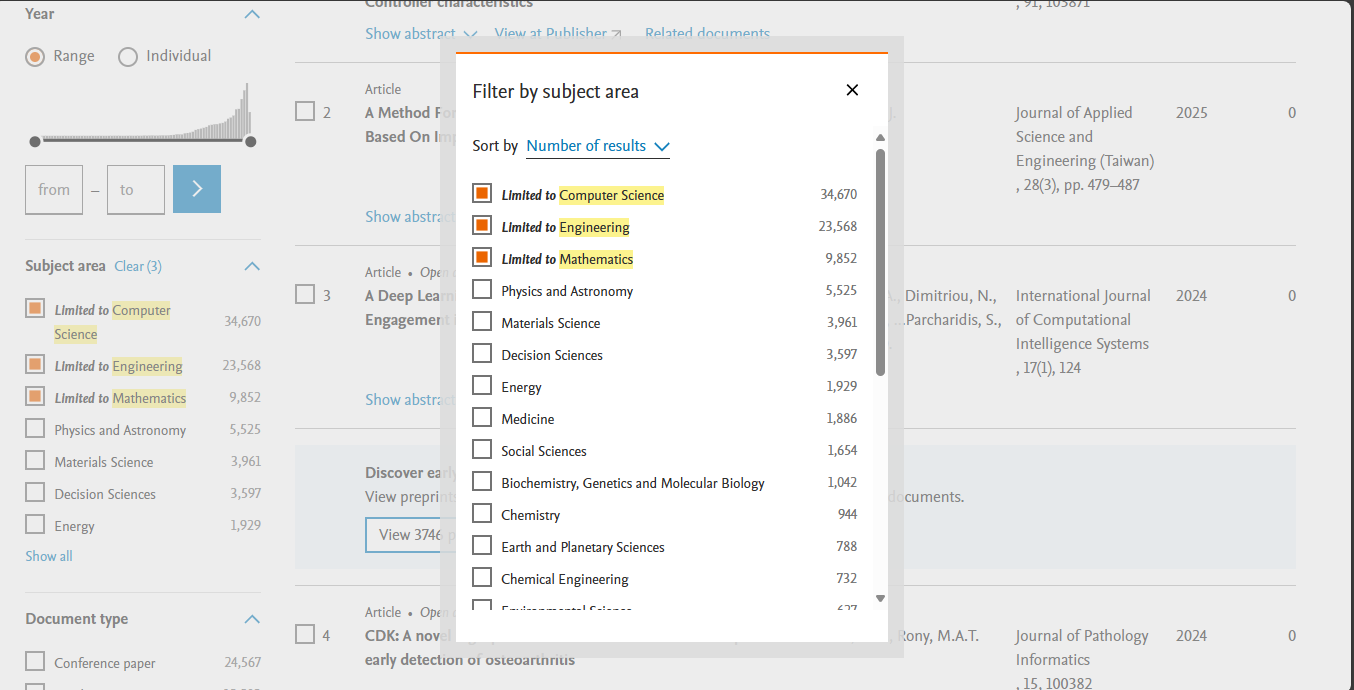
\includegraphics[width=1\linewidth]{1.png}
    \caption{Filtro por area academica:}
    \label{fig:enter-label}
\end{figure}
\subsection{Filtro por tipo de documento}


 Este filtro es esencial porque permite a los investigadores enfocar sus busquedas 
en formatos especıficos, como artıculos de investigacion, revi-
siones o conferencias. Esto mejora la relevancia de los resultados, ahorra tiempo y asegura que se obtenga la informacion
mas adecuada y de calidad para sus necesidades academicas
o cientıficas
\begin{figure}[H]
    \centering
    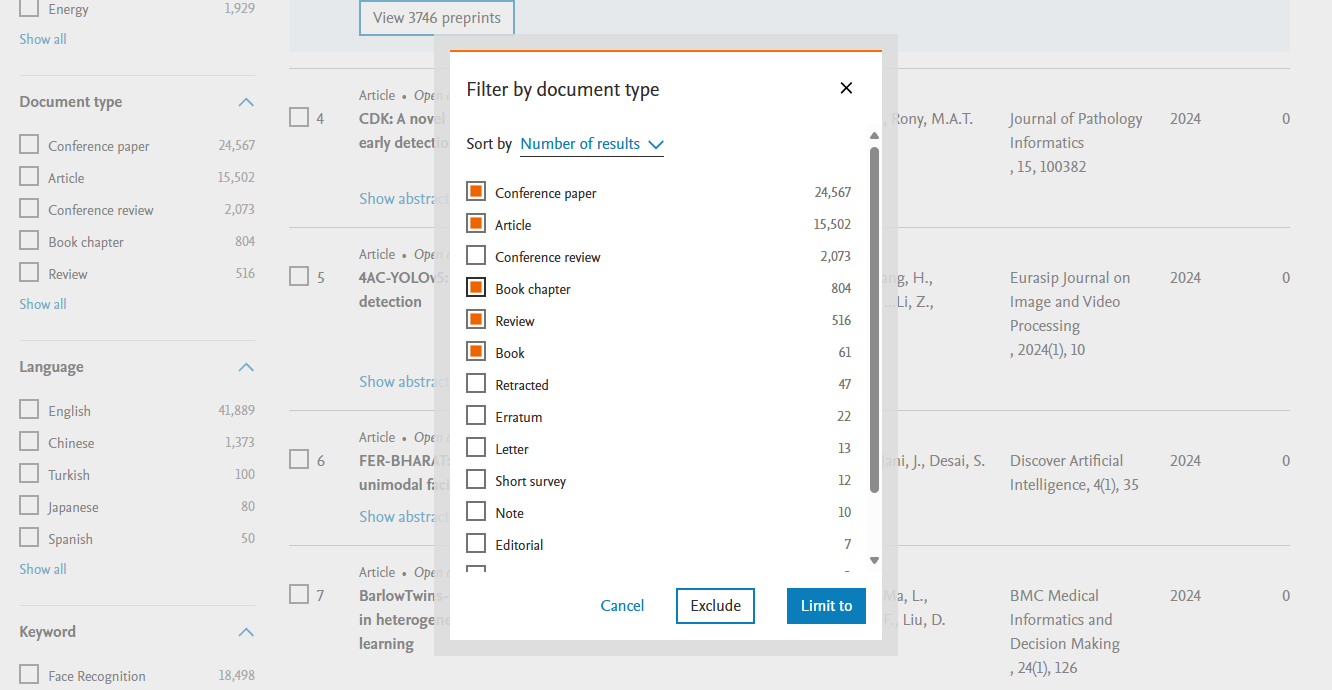
\includegraphics[width=1\linewidth]{2.png}
    \caption{Filtro por tipo de documento}
    \label{fig:enter-label}
\end{figure}


\subsection{Filtro por idioma}

Para nuestro caso elegiremos
los idiomas ingles y espanol, el primero porque es el idioma ˜
mas relevante y en el que mas documentos se publican y el
segundo es un buen agregado ya que manejamos el idioma,
si bien los documentos escritos espanol no estan en la misma ˜
cantidad que los escritos en ingles, podriamos omitir grandes
hallazgos que nos beneficien.
\begin{figure}[h]
    \centering
    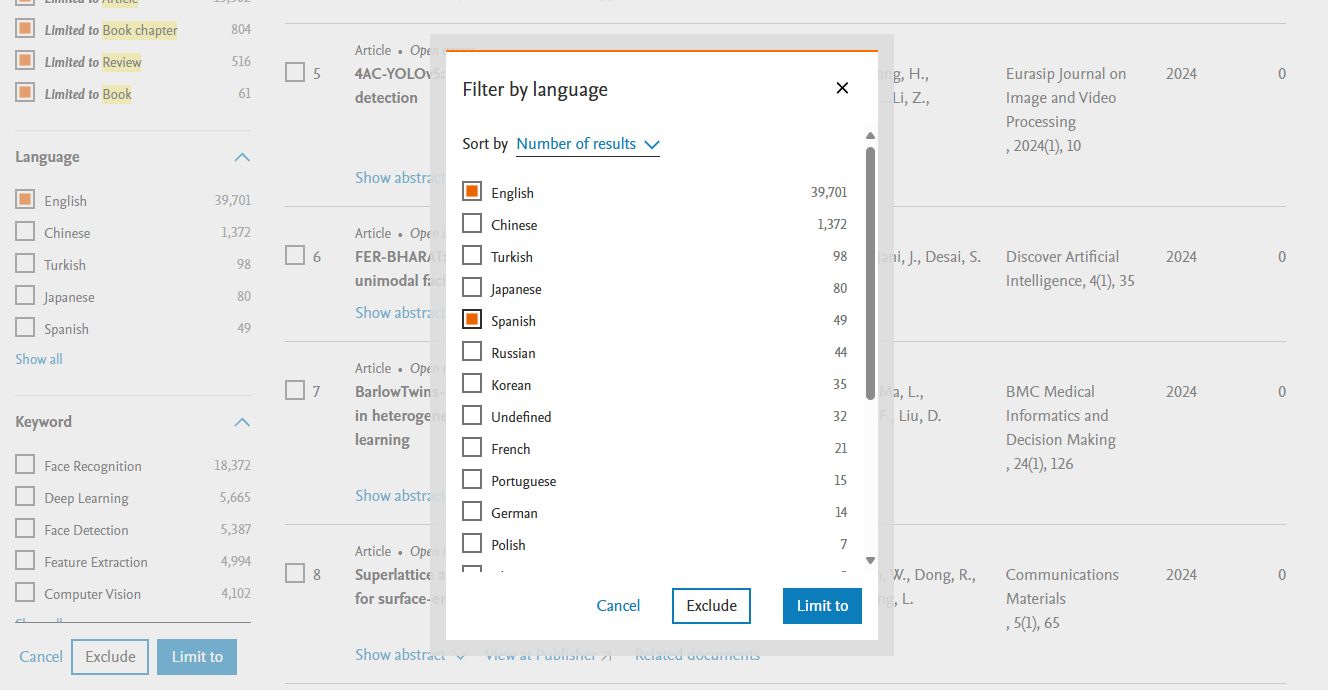
\includegraphics[width=1\linewidth]{3.png}
    \caption{ Filtro por idioma}
    \label{fig:enter-label}
\end{figure}
\subsection{Filtro por palabras clave}

Se eligieron un total de
30 palabras claves, de las cuales solo cuatro cumplen con los
filtros que elegimos anteriormente, disminuyendo la cantidad
de documentos a un total de 27,943. Con esta cifra y por
sobre todo las cuatro palabras clave que se encontraron en
los dumentos, podemos deternernos y empezar con el analisis
bibliografico para determinar si hay un documento que cumpla
con nuestra busqueda ya que, de las palabras claves seleccionadas de las cuales no se encontraron documentos, tenemos
’Optimization’,’Facial expression recognition’, ’Students’ y
’Gesture recognition’.
\begin{figure}[H]
    \centering
    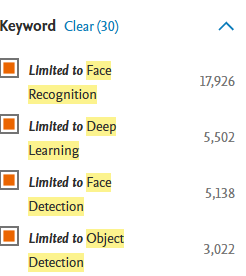
\includegraphics[width=0.5\linewidth]{4.png}
    \caption{Filtro por palabras clave}
    \label{fig:enter-label}
\end{figure}

\section{RESULTADOS DEL ANALISIS}

El query resultante de todos estos filtros:
TITLE-ABS-KEY ( face AND detection)
AND ( LIMIT-TO ( SUBJAREA , C¸ OMP”) OR LIMIT-TO (
SUBJAREA , .ENGI”) OR LIMIT-TO ( SUBJAREA , ”MATH”)
) AND ( LIMIT-TO ( DOCTYPE , c¸p”) OR LIMIT-TO (
DOCTYPE , .a
r”) OR LIMIT-TO ( DOCTYPE , re”) OR
LIMIT-TO ( DOCTYPE , c¸h”) ) AND ( LIMIT-TO ( LANGUAGE , .English”) ) AND ( LIMIT-TO ( EXACTKEYWORD
, ”Face Recognition”) OR LIMIT-TO ( EXACTKEYWORD ,
”Deep Learning”) )
\subsection{analisis periodos 2013-2018 a 2019-2024}
en este apartado mostaremos los resultados de los diferentes periodos de tiempo y analisaremos sus diferencias

\subsection{analisis incial}
Al realizar la consulta inicial, pero limitando los periodos de tiempo a intervalos de 5 años, podremos observar los resultados específicos de cada uno de estos períodos a continuación.
\begin{figure}[H]
    \centering
    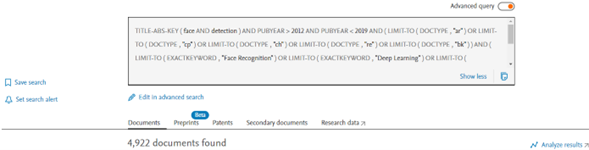
\includegraphics[width=1\linewidth]{resultados 2013.png}
    \caption{resultados 2013 a 2018}
    \label{fig:enter-label}
\end{figure}
\begin{figure}[H]
    \centering
    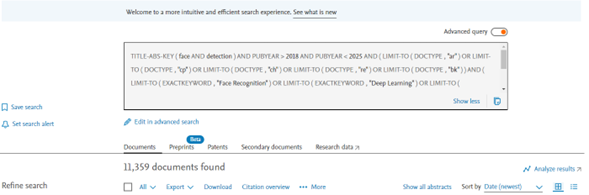
\includegraphics[width=1\linewidth]{resultados 2019.png}
    \caption{resultados 2019 a 2024}
    \label{fig:enter-label}
\end{figure}

como se puede observar la diferencia e articulos es de mas del doble, esto quiere decir que en los ultimos 5 años el aumento de articulos publicados es exponencial a comparacion de los 5 años anteriores a este periodo.

\subsection{grafica titulos}
en este apartado podremos observar las graficas donde se analisan los titulos 
\begin{figure}[H]
    \centering
    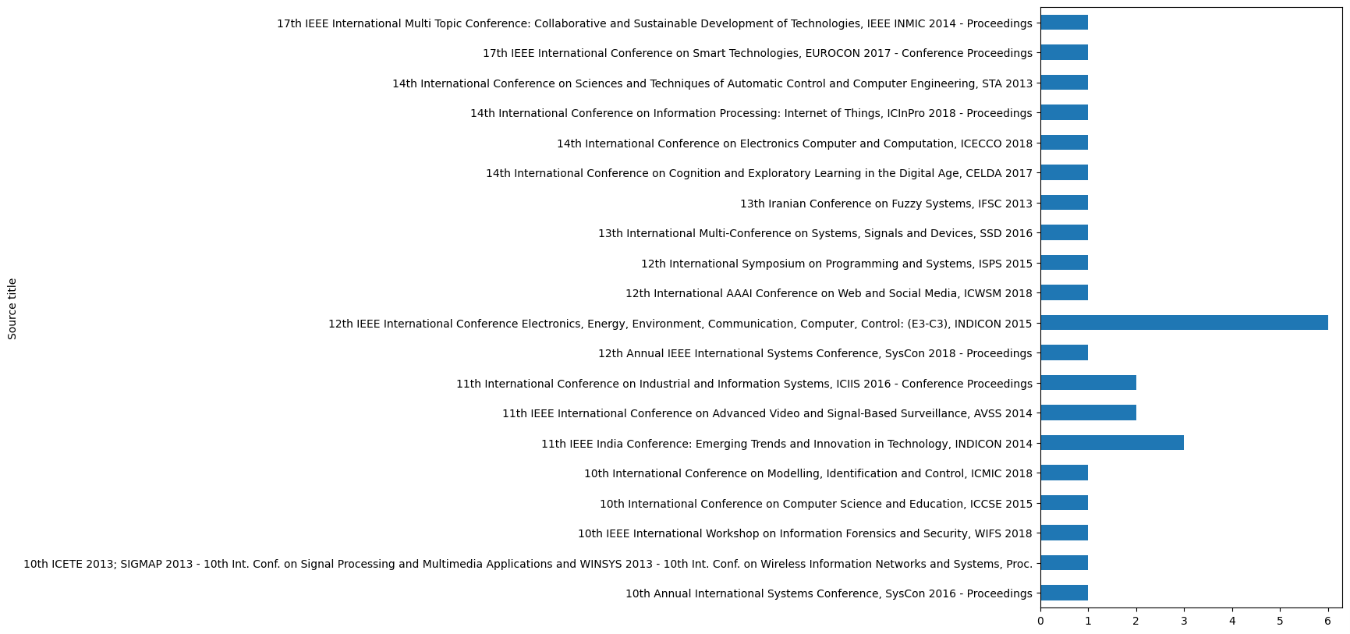
\includegraphics[width=1\linewidth]{titulos2013.png}
    \caption{resultados 2013 a 2018}
    \label{fig:enter-label}

\subsubsection{Periodo 2013-2018:}
Durante este tiempo, hubo menos artículos o títulos publicados.
La gráfica muestra un solo título que destaca por encima de los demás.
\end{figure}
\begin{figure}[H]
    \centering
    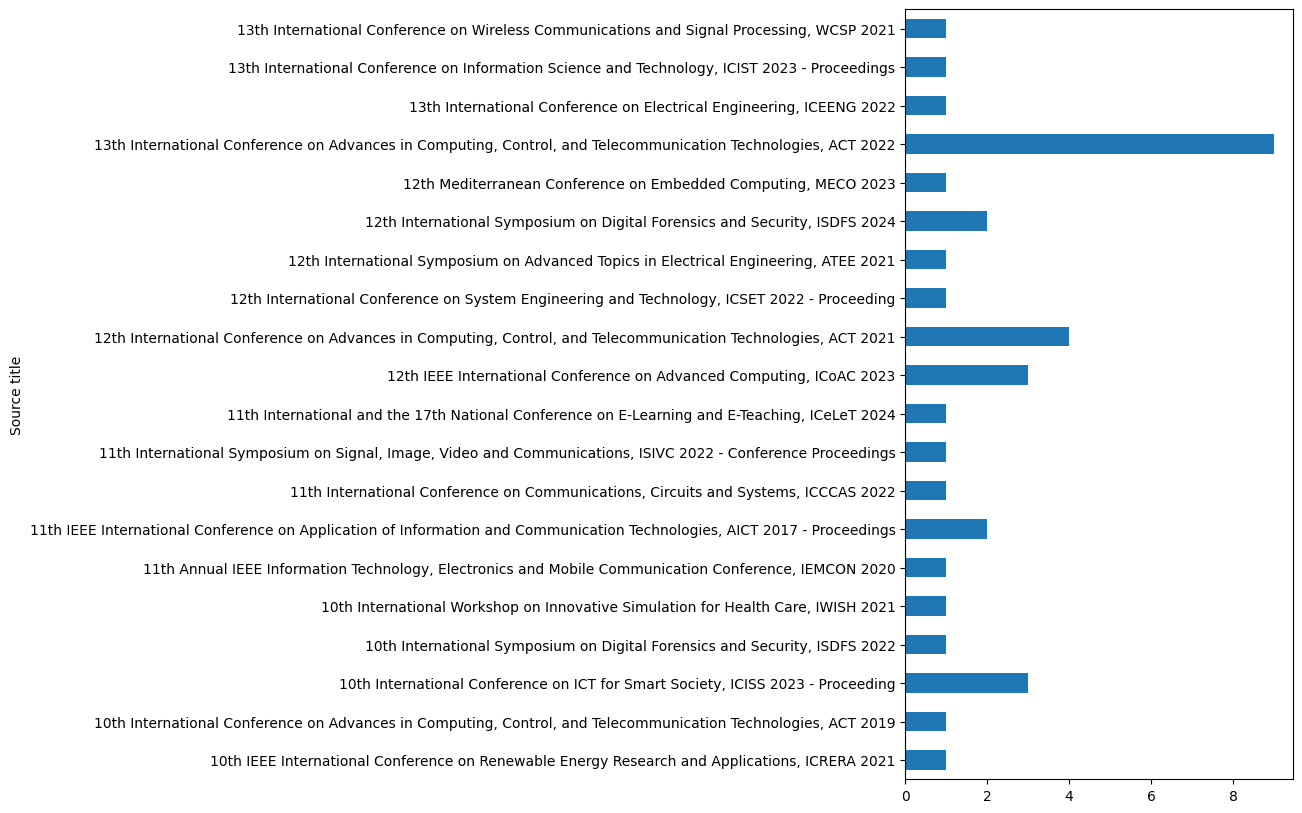
\includegraphics[width=1\linewidth]{titulos2019.png}
    \caption{resultados 2019 a 2024}
    \label{fig:enter-label}
\end{figure}
\subsubsection{Periodo 2019-2024:}
En contraste, en este periodo, se ha incrementado el número de temas o títulos publicados.
La gráfica muestra títulos un poco más grandes, lo que sugiere un crecimiento en la cantidad de publicaciones.


\subsection{grafica Fuentes con mas articulos}
\subsubsection{Periodo 2013-2018:}
En esta gráfica, destaca un tema en particular: “Lecture Notes in Computer Science”, que cuenta con poco más de 300 artículos.
Le sigue “Proceedings of SPIE”, con menos de 150 artículos.
Durante este periodo, un solo tema sobresale por encima de los demás, siendo “Lecture Notes in Computer Science” más del doble que cualquier otro.
\begin{figure}[H]
    \centering
    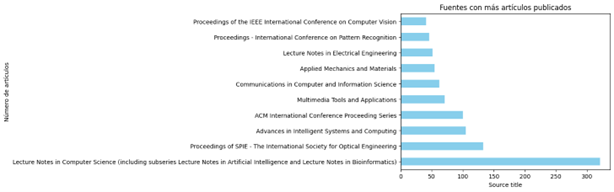
\includegraphics[width=1\linewidth]{fuentes2013.png}
    \caption{resultados 2013 a 2018}
    \label{fig:enter-label}
\end{figure}


\subsubsection{Periodo 2019-2024:}
En este periodo, el interés en estos temas aumentó exponencialmente.
“Lecture Notes in Computer Science” sigue siendo el tema destacado, con alrededor de 350 artículos.
Sin embargo, ahora hay más diversidad: “IEEE ACCESS” tiene más de 325 artículos, y “ACM International Conference” supera los 250.

\begin{figure}[H]
    \centering
    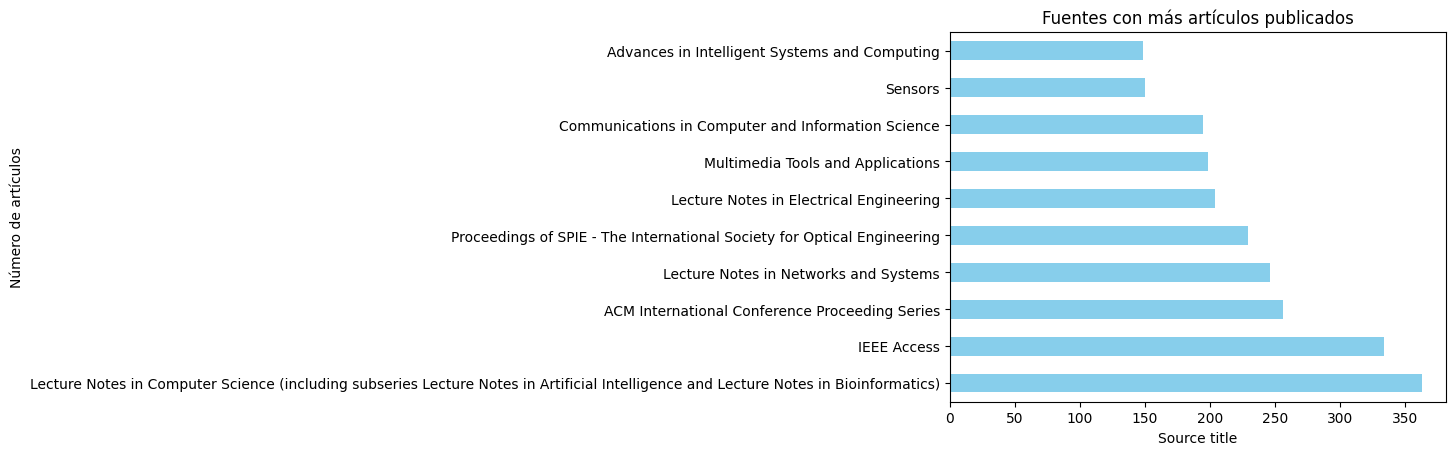
\includegraphics[width=1\linewidth]{fuentes2019.png}
    \caption{resultados 2019 a 2024}
    \label{fig:enter-label}
\end{figure}

\subsection{grafica frecuencia de palabras}
\subsubsection{Periodo 2013-2018:}
La palabra “detección” tenía la frecuencia más alta, con un valor de 2180, ocupando el primer lugar.
Otras palabras relevantes incluían “rostro”, “reconocimiento”, “uso”, “basado”, “aprendizaje”, “profundo”, “imágenes” y “algoritmo”.
\begin{figure}[H]
    \centering
    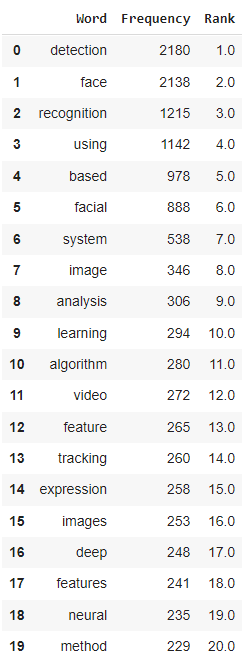
\includegraphics[width=0.4\linewidth]{frecuenciapalabrastitulos2013.png}
    \caption{resultados 2013 a 2018}
    \label{fig:enter-label}
\end{figure}
\subsubsection{Periodo 2019-2024:}
La palabra “detección” sigue siendo la más frecuente, con un valor de 5191.
Además, aparecen términos como “usando”, “reconocimiento”, “basado”, “aprendizaje”, “profundo”, “sistema”, “red neuronal” y “tiempo real”.
\begin{figure}[H]
    \centering
    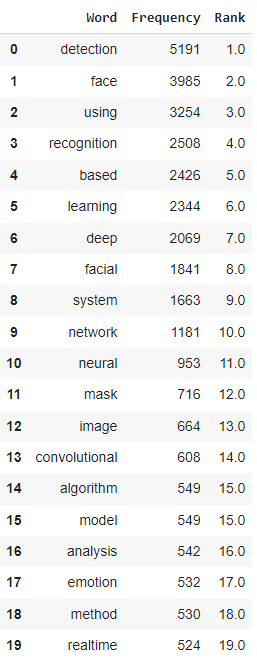
\includegraphics[width=0.4\linewidth]{frecuencia2019.png}
    \caption{resultados 2019 a 2024}
    \label{fig:enter-label}
\end{figure}
\subsection{grafica nube de palabras}

\subsubsection{Periodo 2013-2018:}

En esta visualización, se destacan términos relacionados con la tecnología de reconocimiento facial, como “detección”, “rostro”, “reconocimiento”, “expresión” y “algoritmo”. La variación en el tamaño de las palabras indica su frecuencia o importancia en el contexto.
\begin{figure}[H]
    \centering
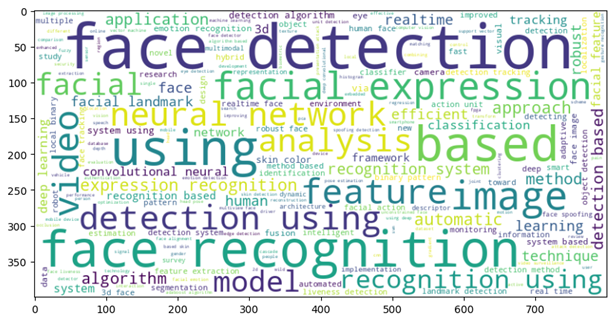
\includegraphics[width=1\linewidth]{nube2013.png}
    \caption{resultados 2013 a 2018}
    \label{fig:enter-label}
\end{figure}

\subsubsection{Periodo 2019-2024:}
En esta nube de palabras, los términos más prominentes están relacionados con inteligencia artificial, visión por computadora y aprendizaje automático. Algunas palabras clave son “reconocimiento facial”, “aprendizaje profundo” y “red neuronal”. También aparecen términos como “detección”, “algoritmo”, “expresión facial” y “convolucional”.
\begin{figure}[H]
    \centering
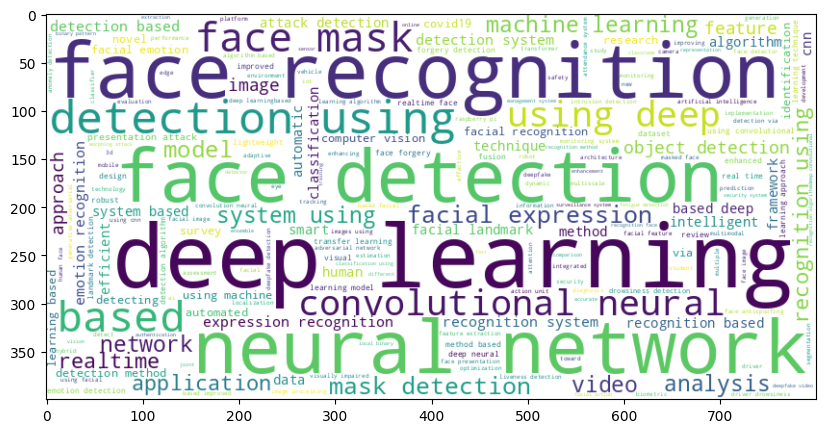
\includegraphics[width=1\linewidth]{nube2019.png}
    \caption{resultados 2019 a 2024}
    \label{fig:enter-label}
\end{figure}
\subsection{grafica palabras clave por titulo}

\subsubsection{Periodo 2013-2018:}
Durante este periodo, la investigación de palabras clave se centró en términos relacionados con la tecnología de reconocimiento facial, detección de partes faciales, seguimiento en tiempo real y otros temas afines1.
Algunos títulos destacados incluyeron:
“Detección robusta en tiempo real y seguimiento de rostros mediante funciones extendidas de Haar y algoritmo de mejora.”
“Detección de partes faciales a través del modelo de partes deformables con anotación de partes.”
“Análisis de fotogramas clave acelerado por GPU para detección de rostros en videos.”
\begin{figure}[H]
    \centering
    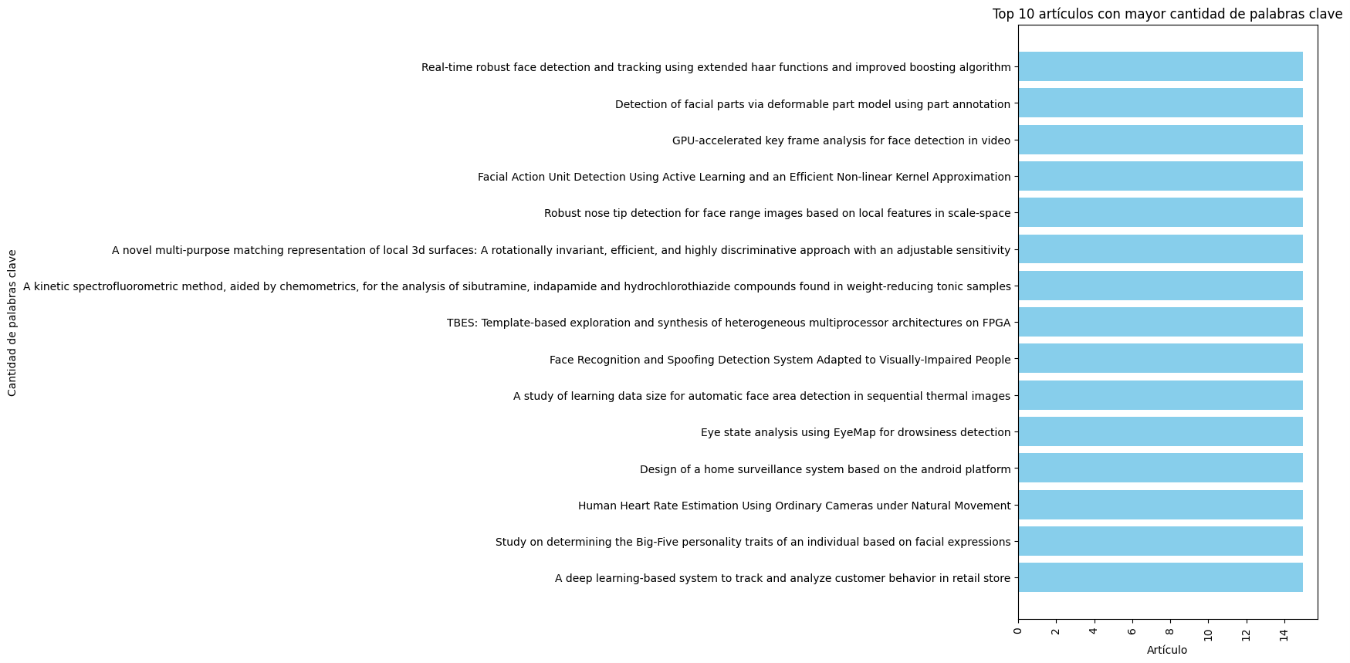
\includegraphics[width=1\linewidth]{palabrasclavetitulos2013.png}
    \caption{resultados 2013 a 2018}
    \label{fig:enter-label}
\end{figure}

\subsubsection{Periodo 2019-2024:}
En este periodo, la investigación de palabras clave se amplió para incluir temas más diversos relacionados con inteligencia artificial, visión por computadora y aprendizaje automático1.
Algunos títulos relevantes fueron:
“Detección de máscaras faciales con control de entrada de puertas automatizado mediante redes neuronales convolucionales.”
“Identificación innovadora de expresiones faciales para investigaciones criminales mediante aprendizaje no supervisado y comparación de precisión con clasificadores CNN.”
\begin{figure}[H]
    \centering
    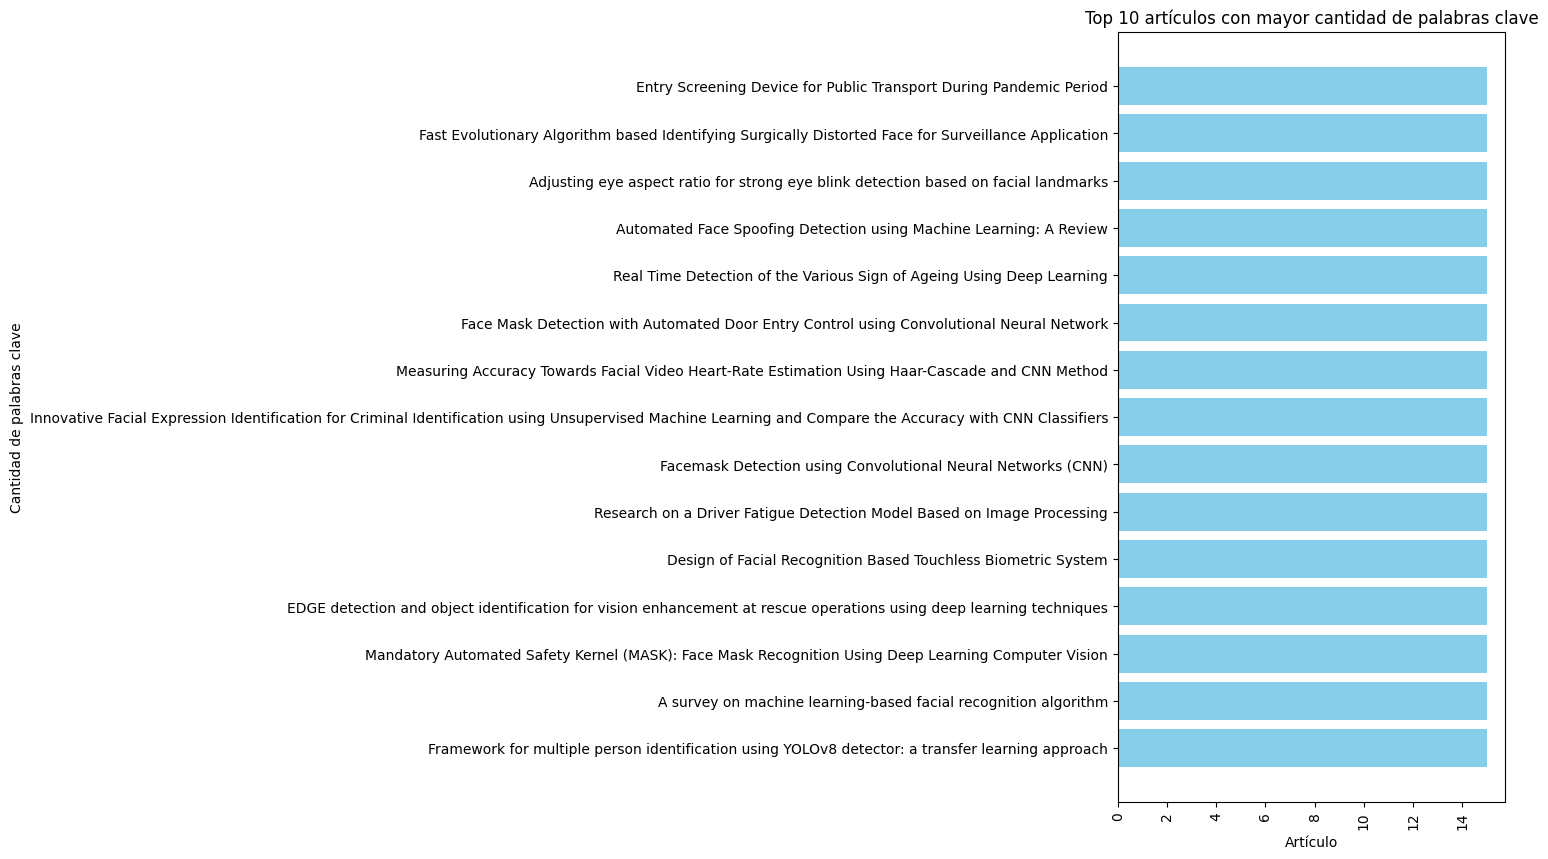
\includegraphics[width=1\linewidth]{palabrasclavetitulos2019.png}
    \caption{resultados 2019 a 2024}
    \label{fig:enter-label}
\end{figure}
\section{Mapas de Categorías Gramaticales}
En esta sección, realizaremos un análisis de la estructura gramatical presente en los resúmenes (abstracts) y los títulos de los documentos. Para este propósito, hemos seleccionado el período de tiempo comprendido entre 2019 y 2024. A fin de garantizar la precisión y confiabilidad del análisis, utilizamos la biblioteca Spacy. Esta herramienta nos permite desglosar y etiquetar las palabras en las frases de manera más exhaustiva, lo que facilita la identificación de patrones gramaticales y tendencias en los textos. Así, obtendremos una comprensión más profunda de cómo se estructuran lingüísticamente los resúmenes y títulos dentro de nuestro conjunto de datos.
\subsection{Frecuencia de categorias gramaticales en los titulos}
\begin{figure}[H]
    \centering
    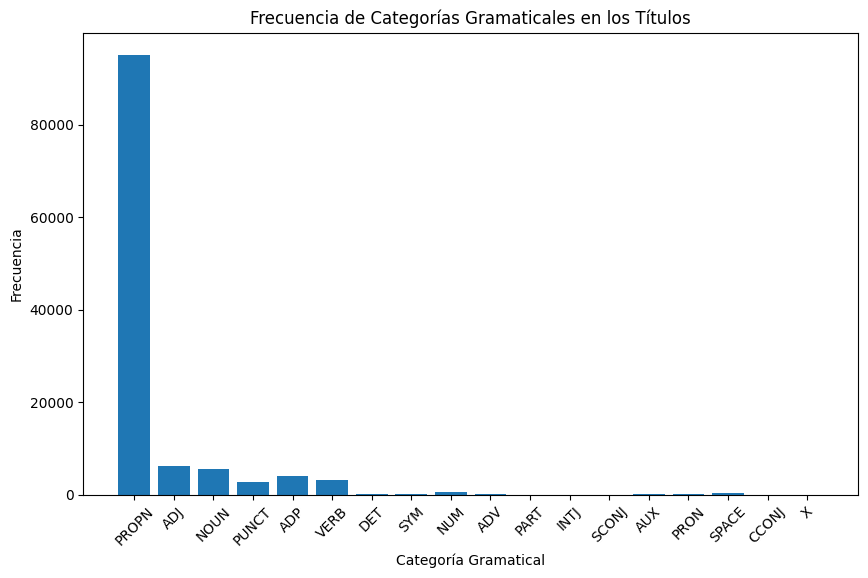
\includegraphics[width=1\linewidth]{mapaTitulos.png}
    \caption{Enter Caption}
    \label{fig:enter-label}
\end{figure}

La gráfica es un histograma de barras titulado “Frecuencia de Categorías Gramaticales en los Títulos”.
En el eje x, se encuentran diferentes categorías gramaticales, como sustantivos propios (PROPN), adjetivos (ADJ), puntuación (PUNCT), preposiciones (ADP), verbos auxiliares (AUX), conjunciones coordinantes (CCONJ), determinantes (DET), números (NUM), partículas (PART), pronombres (PRON), conjunciones subordinantes (SCONJ), símbolos (SYM) y otras categorías abreviadas de manera similar.
El eje y representa la frecuencia, con valores que van desde 0 hasta 80000 en incrementos de 10000.
La categoría gramatical más frecuente es “PROPN” (sustantivos propios), con una frecuencia cercana a 80000. Esto indica que los sustantivos propios son la categoría más común en los títulos de este conjunto de datos. Las demás categorías tienen frecuencias significativamente más bajas.
\subsection{Frecuencia de categorias gramaticales en los abstracts}
\begin{figure}[H]
    \centering
    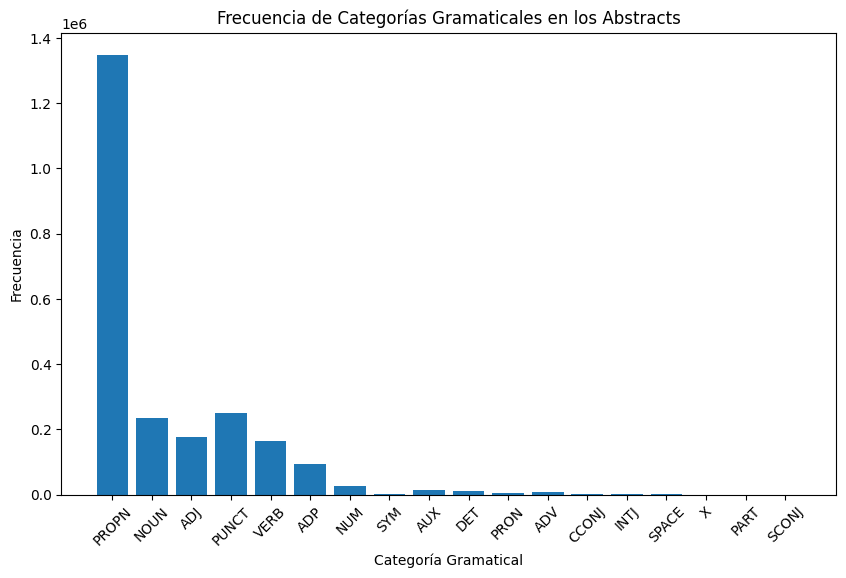
\includegraphics[width=1\linewidth]{mapaabstract.png}
    \caption{Enter Caption}
    \label{fig:enter-label}
\end{figure}
La gráfica muestra un histograma de barras titulado “Frecuencia de Categorías Gramaticales en los Abstracts”.
En el eje x, se encuentran diferentes categorías gramaticales, como pronombres (PRON), sustantivos (NOUN), adjetivos (ADJ), puntuación (PUNCT), verbos (VERB), determinantes (DET), preposiciones (ADP), números (NUM), conjunciones (CONJ), adverbios (ADV) y símbolos (SYM).
El eje y representa la frecuencia, con valores que van desde 0 hasta 1e6 en incrementos.
La categoría gramatical más frecuente en los abstracts es “PRON” (pronombre), lo que indica que los pronombres son ampliamente utilizados en este tipo de texto. Las demás categorías tienen frecuencias más bajas.

\section{conclusiones}

\subsection{Tendencia de Publicaciones:}
Durante el periodo de 2013 a 2018, hubo menos artículos o títulos publicados.\\
Sin embargo, en el periodo de 2019 a 2024, se observa un aumento significativo en la cantidad de publicaciones.\\
“Lecture Notes in Computer Science” es una fuente destacada en ambos periodos.

\subsection{Diversidad de Temas:}
En el periodo de 2019 a 2024, se amplió la investigación para incluir temas más diversos relacionados con inteligencia artificial, visión por computadora y aprendizaje automático.\\
Aunque “Lecture Notes in Computer Science” sigue siendo el tema destacado, ahora también hay más diversidad, como “IEEE ACCESS” y “ACM International Conference”.

\subsection{Diferencia entre los periodos de tiempo:}
al hacer la primera busqueda y limitar los periodos de tiempo pudimos observar la diferencia abismal entre ambos periodos de tiempo, desde un principio ya teniamos una idea de que podriamos observar en el analisis de las graficas, pero aun asi es muy interesante ver los cambios en las tendencias y el mayor interes en la gente para investigar el tema de la inteligencia artificial y el reconocimiento facial, fortaleciendo la idea de que el futuro este sera un campo muy importante en la ingeniera y computacion.
\section{Referencias}

\begin{enumerate}
    \item M. H. Wasim Khan, “An unsupervised deep learning ensemble model for anomaly detection in static attributed social networks,” International Journal of Cognitive Computing in Engineering, vol. 3, no. 1, pp. 153 – 160, 2022.

    \item H. Bouma, R. Pruim, A. V. Rooijen, J.-M. ten Hove, J. van Mil, and B. Kromhout, “Document anonymization for border guards and immigration services,” in Counterterrorism, Crime Fighting, Forensics, and Surveillance Technologies IV, H. Bouma, R. Prabhu, R. J. Stokes, and Y. Yitzhaky, Eds., vol. 11542, International Society for Optics and Photonics. SPIE, 2020, p. 115420C. [Online]. Available: https://doi.org/10.1117/12.2571944

    \item A. Khodabakhsh and H. Loiselle, “Action-independent generalized behavioral identity descriptors for look-alike recognition in videos,” in 2020 International Conference of the Biometrics Special Interest Group (BIOSIG), 2020, pp. 1–6.
\end{enumerate}

\bibliographystyle{IEEEtran}


\end{document}

